\documentclass[tikz]{standalone}
\usetikzlibrary{positioning}

\begin{document}
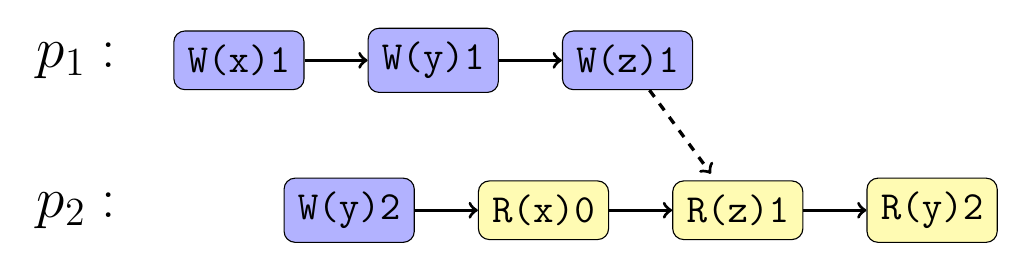
\begin{tikzpicture}
\tikzset{
  wop/.style = {rectangle, rounded corners, fill = blue!30, draw, font = \Large, inner sep = 5pt},
  rop/.style = {rectangle, rounded corners, fill = yellow!30, draw, font = \Large, inner sep = 5pt}, process/.style = {font = \huge}, po/.style = {->, very thick},
  rw/.style = {->, shorten >= 3pt, very thick, dashed},
  vis/.style = {->, shorten >= 3pt, very thick, dashed}
}

  \node (p1) [process] {$p_1:$};
  \node (wx1) [wop, right = 0.6cm of p1] {\texttt{W(x)1}};
  \node (wy1) [wop, right = 0.8cm of wx1] {\texttt{W(y)1}};
  \node (wz1) [wop, right = 0.8cm of wy1] {\texttt{W(z)1}};

  \node (p2) [process, below = 1.2cm of p1] {$p_2:$};
  \node (wy2) [wop, right = 2cm of p2] {\texttt{W(y)2}};
  \node (rx0) [rop, right = 0.8cm of wy2] {\texttt{R(x)0}};
  \node (rz1) [rop, right = 0.8cm of rx0] {\texttt{R(z)1}};
  \node (ry2) [rop, right = 0.8cm of rz1] {\texttt{R(y)2}};

  \draw [po] (wx1) to (wy1);
  \draw [po] (wy1) to (wz1);

  \draw [po] (wy2) to (rx0);
  \draw [po] (rx0) to (rz1);
  \draw [po] (rz1) to (ry2);

  \draw [vis] (wz1) to (rz1);

\end{tikzpicture}
\end{document}
